\begin{tikzpicture}
\begin{axis} [
     title={},
     width=\textwidth,
     height=.25\textheight,
     xlabel={\footnotesize \textbf{Visual Pattern}},
     ylabel={\footnotesize \textbf{Accuracy}},
     bar width = 4pt,
     ybar = .02cm,
     xmin=0.0, xmax=10,
     ymin=0.0, ymax=80,
     x tick label style={font=\tiny},
     y tick label style={font=\tiny},
     xtick={1,2,3,4,5,6,7,8,9},
     xticklabels={Orientation, State, Quantity, Relational Context, Color, Physical Characteristics, Text, Viewpoint, Presence of Features},
     y label style={at={(axis description cs:0.05,.5)},anchor=south},
     ymajorgrids=false,
     xmajorgrids=false,
     legend style={
			at={(0.5,-0.35)},
			anchor=north,
			legend columns=5,
            }
] 

\addplot[color=blue!40, fill=blue, area legend] coordinates{(1, 0.0) (2, 0.0) (3, 0.0) (4, 28.6) (5, 28.6) (6, 0.0) (7, 0.0) (8, 16.7) (9, 40.0)};
\addplot[color=blue!40, fill=blue!60,  area legend] coordinates {(1, 8.3) (2, 0.0) (3, 0.0) (4, 14.3) (5, 7.1) (6, 0.0) (7, 16.7) (8, 8.3) (9, 12.5)};
\addplot[color=blue!40, fill=blue!30,  area legend] coordinates {(1, 8.3) (2, 5.3) (3, 0.0) (4, 7.1) (5, 14.3) (6, 0.0) (7, 16.7) (8, 8.3) (9, 5.0)};
\addplot[color=blue!40, fill=blue!10,  area legend] coordinates {(1, 8.3) (2, 0.0) (3, 0.0) (4, 0.0) (5, 0.0) (6, 0.0) (7, 0.0) (8, 0.0) (9, 0.0)};
\addplot[color=blue!40, fill=blue!2,  area legend] coordinates {(1, 8.3) (2, 10.5) (3, 8.3) (4, 21.4) (5, 21.4) (6, 28.6) (7, 0.0) (8, 0.0) (9, 5.0)};

\addplot[color=red!20, fill=red!20,  area legend] coordinates {(1, 16.7) (2, 31.6) (3, 33.3) (4, 39.3) (5, 71.4) (6, 42.9) (7, 33.3) (8, 16.7) (9, 47.5)};
\addplot[color=red!60, fill=red!60,  area legend] coordinates {(1, 33.3) (2, 5.3) (3, 16.7) (4, 21.4) (5, 64.3) (6, 14.3) (7, 16.7) (8, 16.7) (9, 37.5)};
\addplot[color=red, fill=red,  area legend] coordinates {(1, 8.3) (2, 47.4) (3, 41.7) (4, 53.6) (5, 78.6) (6, 57.1) (7, 50.0) (8, 25.0) (9, 72.5)};

\legend{\textbf{OMG-Llava (7B)}, \textbf{Llava-G (7B)}, \textbf{LISA (7B)}, \textbf{GLaMM (7B)}, \textbf{GLaMM$\dagger$ (7B)}, \textbf{Llava (13B)}, \textbf{Llava (7B)}, \textbf{Cambrian (8B)}}

\end{axis}
\end{tikzpicture}